% Options for packages loaded elsewhere
\PassOptionsToPackage{unicode}{hyperref}
\PassOptionsToPackage{hyphens}{url}
%
\documentclass[
  man,floatsintext]{apa6}
\usepackage{amsmath,amssymb}
\usepackage{lmodern}
\usepackage{iftex}
\ifPDFTeX
  \usepackage[T1]{fontenc}
  \usepackage[utf8]{inputenc}
  \usepackage{textcomp} % provide euro and other symbols
\else % if luatex or xetex
  \usepackage{unicode-math}
  \defaultfontfeatures{Scale=MatchLowercase}
  \defaultfontfeatures[\rmfamily]{Ligatures=TeX,Scale=1}
\fi
% Use upquote if available, for straight quotes in verbatim environments
\IfFileExists{upquote.sty}{\usepackage{upquote}}{}
\IfFileExists{microtype.sty}{% use microtype if available
  \usepackage[]{microtype}
  \UseMicrotypeSet[protrusion]{basicmath} % disable protrusion for tt fonts
}{}
\makeatletter
\@ifundefined{KOMAClassName}{% if non-KOMA class
  \IfFileExists{parskip.sty}{%
    \usepackage{parskip}
  }{% else
    \setlength{\parindent}{0pt}
    \setlength{\parskip}{6pt plus 2pt minus 1pt}}
}{% if KOMA class
  \KOMAoptions{parskip=half}}
\makeatother
\usepackage{xcolor}
\usepackage{longtable,booktabs,array}
\usepackage{calc} % for calculating minipage widths
% Correct order of tables after \paragraph or \subparagraph
\usepackage{etoolbox}
\makeatletter
\patchcmd\longtable{\par}{\if@noskipsec\mbox{}\fi\par}{}{}
\makeatother
% Allow footnotes in longtable head/foot
\IfFileExists{footnotehyper.sty}{\usepackage{footnotehyper}}{\usepackage{footnote}}
\makesavenoteenv{longtable}
\usepackage{graphicx}
\makeatletter
\def\maxwidth{\ifdim\Gin@nat@width>\linewidth\linewidth\else\Gin@nat@width\fi}
\def\maxheight{\ifdim\Gin@nat@height>\textheight\textheight\else\Gin@nat@height\fi}
\makeatother
% Scale images if necessary, so that they will not overflow the page
% margins by default, and it is still possible to overwrite the defaults
% using explicit options in \includegraphics[width, height, ...]{}
\setkeys{Gin}{width=\maxwidth,height=\maxheight,keepaspectratio}
% Set default figure placement to htbp
\makeatletter
\def\fps@figure{htbp}
\makeatother
\setlength{\emergencystretch}{3em} % prevent overfull lines
\providecommand{\tightlist}{%
  \setlength{\itemsep}{0pt}\setlength{\parskip}{0pt}}
\setcounter{secnumdepth}{-\maxdimen} % remove section numbering
% Make \paragraph and \subparagraph free-standing
\ifx\paragraph\undefined\else
  \let\oldparagraph\paragraph
  \renewcommand{\paragraph}[1]{\oldparagraph{#1}\mbox{}}
\fi
\ifx\subparagraph\undefined\else
  \let\oldsubparagraph\subparagraph
  \renewcommand{\subparagraph}[1]{\oldsubparagraph{#1}\mbox{}}
\fi
\newlength{\cslhangindent}
\setlength{\cslhangindent}{1.5em}
\newlength{\csllabelwidth}
\setlength{\csllabelwidth}{3em}
\newlength{\cslentryspacingunit} % times entry-spacing
\setlength{\cslentryspacingunit}{\parskip}
\newenvironment{CSLReferences}[2] % #1 hanging-ident, #2 entry spacing
 {% don't indent paragraphs
  \setlength{\parindent}{0pt}
  % turn on hanging indent if param 1 is 1
  \ifodd #1
  \let\oldpar\par
  \def\par{\hangindent=\cslhangindent\oldpar}
  \fi
  % set entry spacing
  \setlength{\parskip}{#2\cslentryspacingunit}
 }%
 {}
\usepackage{calc}
\newcommand{\CSLBlock}[1]{#1\hfill\break}
\newcommand{\CSLLeftMargin}[1]{\parbox[t]{\csllabelwidth}{#1}}
\newcommand{\CSLRightInline}[1]{\parbox[t]{\linewidth - \csllabelwidth}{#1}\break}
\newcommand{\CSLIndent}[1]{\hspace{\cslhangindent}#1}
\ifLuaTeX
\usepackage[bidi=basic]{babel}
\else
\usepackage[bidi=default]{babel}
\fi
\babelprovide[main,import]{english}
% get rid of language-specific shorthands (see #6817):
\let\LanguageShortHands\languageshorthands
\def\languageshorthands#1{}
% Manuscript styling
\usepackage{upgreek}
\captionsetup{font=singlespacing,justification=justified}

% Table formatting
\usepackage{longtable}
\usepackage{lscape}
% \usepackage[counterclockwise]{rotating}   % Landscape page setup for large tables
\usepackage{multirow}		% Table styling
\usepackage{tabularx}		% Control Column width
\usepackage[flushleft]{threeparttable}	% Allows for three part tables with a specified notes section
\usepackage{threeparttablex}            % Lets threeparttable work with longtable

% Create new environments so endfloat can handle them
% \newenvironment{ltable}
%   {\begin{landscape}\centering\begin{threeparttable}}
%   {\end{threeparttable}\end{landscape}}
\newenvironment{lltable}{\begin{landscape}\centering\begin{ThreePartTable}}{\end{ThreePartTable}\end{landscape}}

% Enables adjusting longtable caption width to table width
% Solution found at http://golatex.de/longtable-mit-caption-so-breit-wie-die-tabelle-t15767.html
\makeatletter
\newcommand\LastLTentrywidth{1em}
\newlength\longtablewidth
\setlength{\longtablewidth}{1in}
\newcommand{\getlongtablewidth}{\begingroup \ifcsname LT@\roman{LT@tables}\endcsname \global\longtablewidth=0pt \renewcommand{\LT@entry}[2]{\global\advance\longtablewidth by ##2\relax\gdef\LastLTentrywidth{##2}}\@nameuse{LT@\roman{LT@tables}} \fi \endgroup}

% \setlength{\parindent}{0.5in}
% \setlength{\parskip}{0pt plus 0pt minus 0pt}

% Overwrite redefinition of paragraph and subparagraph by the default LaTeX template
% See https://github.com/crsh/papaja/issues/292
\makeatletter
\renewcommand{\paragraph}{\@startsection{paragraph}{4}{\parindent}%
  {0\baselineskip \@plus 0.2ex \@minus 0.2ex}%
  {-1em}%
  {\normalfont\normalsize\bfseries\itshape\typesectitle}}

\renewcommand{\subparagraph}[1]{\@startsection{subparagraph}{5}{1em}%
  {0\baselineskip \@plus 0.2ex \@minus 0.2ex}%
  {-\z@\relax}%
  {\normalfont\normalsize\itshape\hspace{\parindent}{#1}\textit{\addperi}}{\relax}}
\makeatother

% \usepackage{etoolbox}
\makeatletter
\patchcmd{\HyOrg@maketitle}
  {\section{\normalfont\normalsize\abstractname}}
  {\section*{\normalfont\normalsize\abstractname}}
  {}{\typeout{Failed to patch abstract.}}
\patchcmd{\HyOrg@maketitle}
  {\section{\protect\normalfont{\@title}}}
  {\section*{\protect\normalfont{\@title}}}
  {}{\typeout{Failed to patch title.}}
\makeatother

\usepackage{xpatch}
\makeatletter
\xapptocmd\appendix
  {\xapptocmd\section
    {\addcontentsline{toc}{section}{\appendixname\ifoneappendix\else~\theappendix\fi\\: #1}}
    {}{\InnerPatchFailed}%
  }
{}{\PatchFailed}
\keywords{chaos, complexity, entropy, tolerance, r, physiology\newline\indent Word count: 925}
\usepackage{lineno}

\linenumbers
\usepackage{csquotes}
\usepackage[titles]{tocloft}
\cftpagenumbersoff{figure}
\renewcommand{\cftfigpresnum}{\itshape\figurename\enspace}
\renewcommand{\cftfigaftersnum}{.\space}
\setlength{\cftfigindent}{0pt}
\setlength{\cftafterloftitleskip}{0pt}
\settowidth{\cftfignumwidth}{Figure 10.\qquad}
\usepackage[labelfont=bf, font={scriptsize, color=gray}]{caption}
\ifLuaTeX
  \usepackage{selnolig}  % disable illegal ligatures
\fi
\IfFileExists{bookmark.sty}{\usepackage{bookmark}}{\usepackage{hyperref}}
\IfFileExists{xurl.sty}{\usepackage{xurl}}{} % add URL line breaks if available
\urlstyle{same} % disable monospaced font for URLs
\hypersetup{
  pdftitle={A New Heuristic Method for the Optimal Selection of Tolerance r for Entropy Indices},
  pdfauthor={Dominique Makowski1},
  pdflang={en-EN},
  pdfkeywords={chaos, complexity, entropy, tolerance, r, physiology},
  hidelinks,
  pdfcreator={LaTeX via pandoc}}

\title{\textbf{A New Heuristic Method for the Optimal Selection of Tolerance \emph{r} for Entropy Indices}}
\author{Dominique Makowski\textsuperscript{1}}
\date{}


\shorttitle{Optimal Tolerance}

\authornote{

Correspondence concerning this article should be addressed to Dominique Makowski, HSS 04-18, 48 Nanyang Avenue, Singapore (\href{mailto:dom.makowski@gmail.com}{\nolinkurl{dom.makowski@gmail.com}}).

}

\affiliation{\vspace{0.5cm}\textsuperscript{1} School of Social Sciences, Nanyang Technological University, Singapore}

\abstract{%
The tolerance threshold \emph{r} is a key parameter of several entropy algorithms (e.g., \emph{SampEn}). Unfortunately, the gold standard method to estimate its optimal value - the one that maximizes \emph{ApEn} - is computationally costly, prompting users to rely to cargo-cult rules-of-thumb such as 0.2 * SD. In this simulation study, we attempted at validating a new heuristic, based on the embedding dimension \emph{m} and the signal's length \emph{n} (optimal \emph{r} = SD * 0.281(\emph{m}-1) + 0.005(log(\emph{n})) - 0.02(\emph{m}-1 * log(\emph{n}))), which was superior to other existing heuristics. All the methods of optimal tolerance \emph{r} estimation used in this study are available in the \emph{NeuroKit2} Python software (Makowski et al., 2021).
}



\begin{document}
\maketitle

\hypertarget{introduction}{%
\subsection{Introduction}\label{introduction}}

Complexity analysis is a growing approach to physiological signals, including cardiac (e.g., Heart Rate Variability, {[}1{]}) and brain activity {[}2{]}. It is an umbrella term for the usage of various complexity indices that quantify concepts such as chaos, entropy, fractal dimension, randomness, predictability, and information. Importantly, some of the most popular indices of entropy (e.g., \emph{ApEn}, \emph{SampEn}, their fuzzy and multiscale variations) and recurrence quantification analysis (RQA), rely on a similar set of parameters. Namely, these are the delay \(\tau\), the embedding dimension \emph{m}, and the tolerance \emph{r}, which are critical to accurately capture the space in which complexity becomes quantifiable. Unfortunately, despite the existence of methods to estimate optimal values for these parameters depending on the signal at hand, their choice often relies on simple heuristics and cargo-cult conventions.

Such is the case of the tolerance threshold \emph{r}, which typically corresponds to the minimal distance required to assigning two points in a state-space as belonging to the same state. It directly impacts the amount of ``recurrences'' of a system and the measure of its tendency to revisit past states, which is the base metric for the calculation of the aforementioned entropy indices. Despite its importance, it is often selected as a function of the standard deviation (SD) of the signal, with (in)famous magic values including \(0.1\) or \(0.2*SD\) {[}3{]}. One of the reason for the longevity of such approach is 1) the past literature (as many past studies used it, it becomes easier to justify the choice of the same values) and 2) the fact that other approaches to estimate the optimal \emph{r} are computationally costly.

The aim of the present study is to investigate the relationship between different methods for optimal tolerance \emph{r} estimation. The ground-truth method used is the tolerance value corresponding to a maximal value of Approximate Entropy - \emph{ApEn} {[}4--6{]}. As this method is computationally expensive, the objective is to see whether any heuristic proxies can be used to satisfyingly approximate \(r_{maxApEn}\).

\hypertarget{methods}{%
\subsection{Methods}\label{methods}}

For \emph{n} = 5760 combinations of different signal types and lengths, as well as noise types and intensities (the procedure used was the same as in {[}7{]}, and the data generation code is available at \textbf{\url{https://github.com/DominiqueMakowski/ComplexityTolerance}}), we computed the Approximate Entropy (\emph{ApEn}), which peak is used to estimate the optimal tolerance level for time-delay embedding spaces ranging from of 1 to 9 embedding dimensions \emph{m}.

The aim of the analysis is to establish a new heuristic based only on the signal's SD and the embedding dimension \emph{m}; and compare all of these approximations with other existing heuristics such as \emph{0.2 SD}, \emph{Chon} {[}6{]}, and the \emph{Schötzel} method (\(1.3334 + 0.5627 * log(dimension)\)) implemented in the package \emph{nolds} {[}8{]}.

\hypertarget{results}{%
\subsection{Results}\label{results}}

\hypertarget{maximum-approximate-entropy}{%
\subsubsection{Maximum Approximate Entropy}\label{maximum-approximate-entropy}}

\begin{figure}
\centering
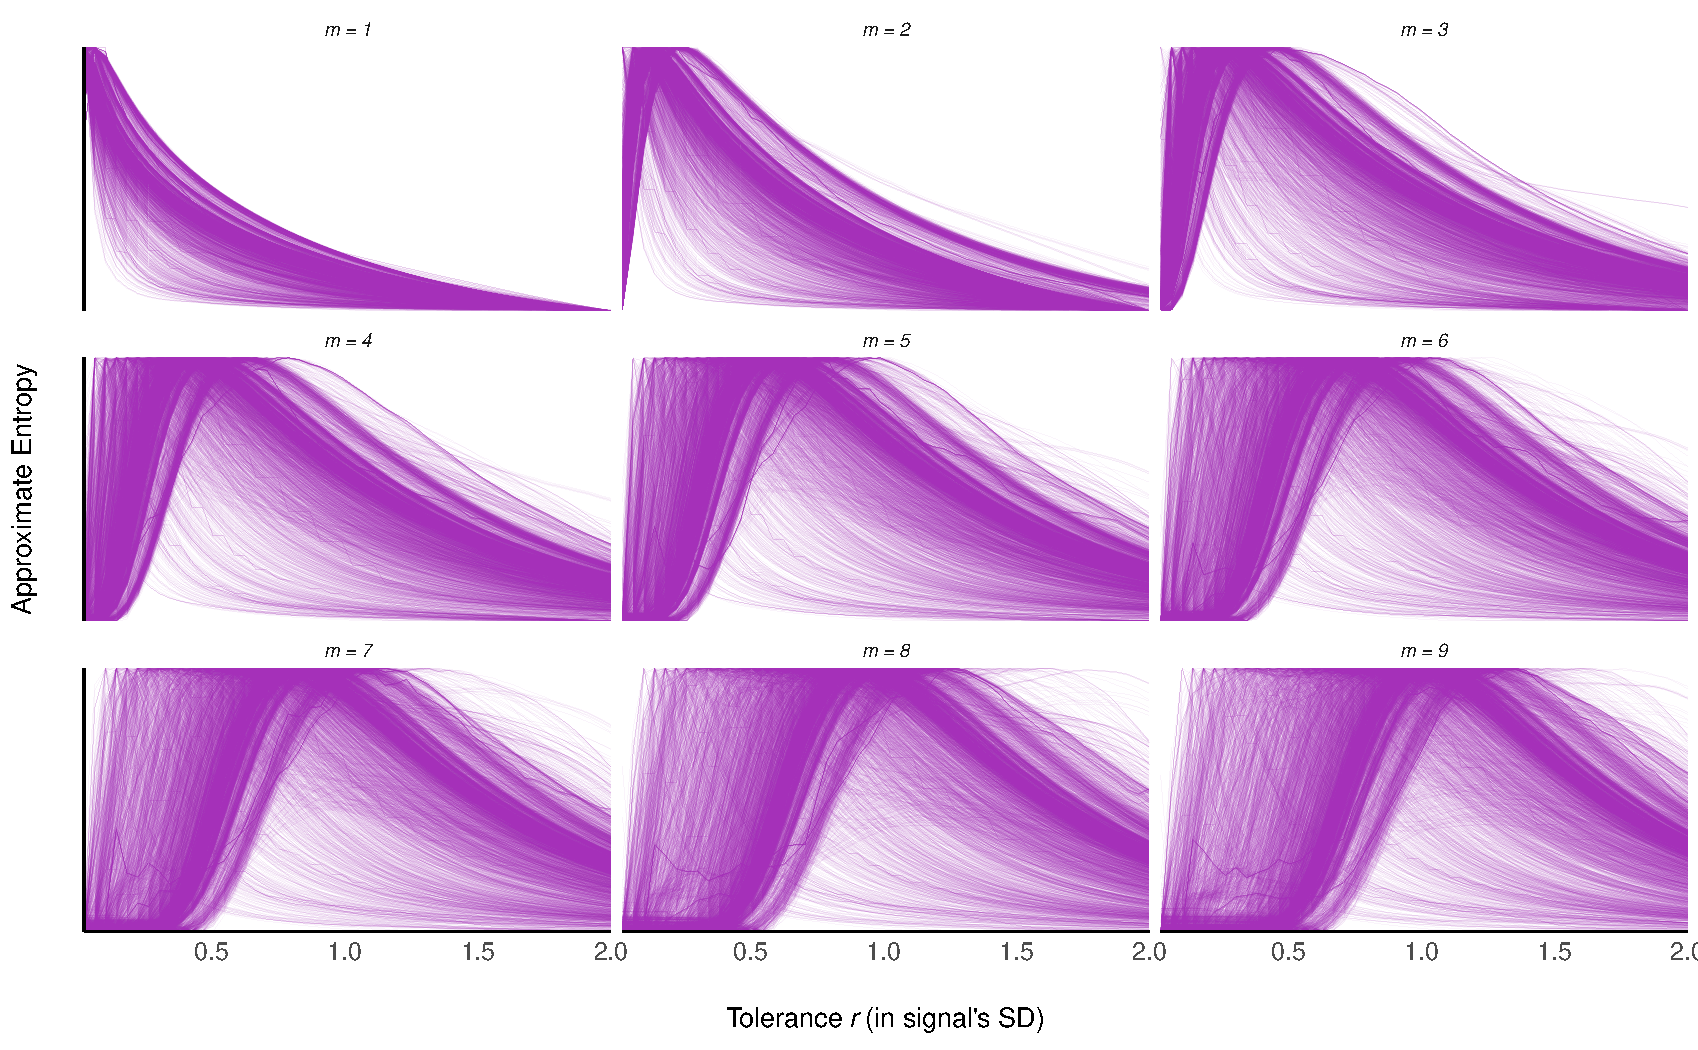
\includegraphics{figures/unnamed-chunk-3-1.pdf}
\caption{\label{fig:unnamed-chunk-3}Approximate Entropy \emph{ApEn} as a function of tolerance \emph{r} (expressed in signal SD) and embedding dimension \emph{m}.}
\end{figure}

\textbf{Figure 1} shows the normalized value of Approximate Entropy \emph{ApEn}
as a function of tolerance \emph{r} and embedding dimension \emph{m}. As expected, the value of \emph{ApEn} peaks at certain values of \emph{r} (hence its usage as an indicator of the optimal tolerance). The location of this peak seems strongly impacted by the embedding dimension \emph{m}, getting more variable - and on average larger - as \emph{m} increases.

\hypertarget{new-heuristic}{%
\subsubsection{New Heuristic}\label{new-heuristic}}

\begin{figure}
\centering
\includegraphics{figures/fig2-1.pdf}
\caption{\label{fig:fig2}Optimal tolerance values approximated by a new heuristic model based on the embedding dimension \emph{m} and the signal length \emph{n} (in samples). The density plots show the true optimal tolernace values as based on max. ApEn.}
\end{figure}

Selecting the tolerance based on the signal's SD alone makes hardly sense, as the embedding dimension has a strong impact on it. In order to validate a new heuristic to approximate the optimal \emph{r} value based on the embedding dimension \emph{m} and the signal's length, we compared different regression specifications using the BIC-based Bayes Factor test. The model including the log-transformed signal length (in samples) and the embedding dimension \emph{m} minus 1 (with no intercept) performed significantly better (\(BF_{10} > 1000\)) than any other version, with an explained variance of 92.64\%. Based on this simple regression model, we can derive the following approximation (assuming a standardized signal with an SD of 1):

\begin{equation}
\widehat{r} = 0.2811(m-1) + 0.0049(\log(n)) - 0.02(m-1 \times \log(n))
\end{equation}

It is to note that shorter signals require larger tolerance values, and the impact of length lowers as the signal gets longer. Also, for a dimension \emph{m} of 2 (and short signal lengths), this equation returns close results to the \emph{0.2 SD} heuristic, which is not entirely surprising as the latter was initially derived under such conditions (that are typical of some applications, such as heart-rate intervals).

\hypertarget{heuristics-comparison}{%
\subsubsection{Heuristics Comparison}\label{heuristics-comparison}}

\begin{longtable}[]{@{}lccc@{}}
\caption{Comparison of Model Performance Indices}\tabularnewline
\toprule()
Model & BIC & R2 & BF \\
\midrule()
\endfirsthead
\toprule()
Model & BIC & R2 & BF \\
\midrule()
\endhead
Makowski & -41375.73 & 0.77 & 1.00 \\
Scholzel & -24637.03 & 0.68 & 0.00e+00 \\
Chon & 24614.17 & 0.18 & 0.00e+00 \\
SD & 35119.90 & 0.00 & 0.00e+00 \\
\bottomrule()
\end{longtable}

We compared together different methods to approximate \(r_{maxApEn}\) (see \textbf{Table 1}) by comparing \(r_{maxApEn}\) (our ground-truth) to the value estimated by different methods. Our heuristic method presented in this study, based on the signal's SD, the embedding dimension and the log-transformed length, surpassed any other models (\(BF_{10} > 1000\), \(R^2\) = 0.77), and was followed by the \emph{Schötzel} adjustment (\(R^2\) = 0.68).

\hypertarget{discussion}{%
\subsection{Discussion}\label{discussion}}

The tolerance threshold \emph{r} is a key parameter of several entropy algorithms, including widely popular ones like \emph{SampEn}. The current gold standard method to estimate the optimal \emph{r} is to compute Approximate Entropy (\emph{ApEn}) over a range of different \emph{r} values and to select the one corresponding to the maximum \emph{ApEn} value. Unfortunately, this method is computationally costly.

In this study, we have shown that a simple heuristic approximation based on the embedding dimension \emph{m} and the log-transformed signal length was a valid approximation of \(r_{maxApEn}\), showing superior performance to other heuristic methods.
We suggest the use of this method as a default alternative to the \emph{0.2 SD} rule of thumb.

While we believe that our data generation procedure was able to generate a wide variety of signals, and that our results are to some extent generalizable, future studies could attempt at refining the estimation procedures for specific signals (for instance, EEG, or heart rate data). All the methods of optimal tolerance \emph{r} estimation used in this study, including our new proposal, are available in the \emph{NeuroKit2} open-source Python software, \texttt{complexity\_tolerance()} function {[}9{]}.

\newpage

\hypertarget{references}{%
\subsection{References}\label{references}}

\hypertarget{refs}{}
\begin{CSLReferences}{0}{0}
\leavevmode\vadjust pre{\hypertarget{ref-pham2021heart}{}}%
\CSLLeftMargin{1. }%
\CSLRightInline{Pham, T.; Lau, Z.J.; Chen, S.; Makowski, D. Heart Rate Variability in Psychology: A Review of HRV Indices and an Analysis Tutorial. \emph{Sensors} \textbf{2021}, \emph{21}, 3998.}

\leavevmode\vadjust pre{\hypertarget{ref-lau2021brain}{}}%
\CSLLeftMargin{2. }%
\CSLRightInline{Lau, Z.J.; Pham, T.; Annabel, S.; Makowski, D. Brain Entropy, Fractal Dimensions and Predictability: A Review of Complexity Measures for EEG in Healthy and Neuropsychiatric Populations. \textbf{2021}.}

\leavevmode\vadjust pre{\hypertarget{ref-pincus1992approximate}{}}%
\CSLLeftMargin{3. }%
\CSLRightInline{Pincus, S.M.; Viscarello, R.R. Approximate Entropy: A Regularity Measure for Fetal Heart Rate Analysis. \emph{Obstetrics and gynecology} \textbf{1992}, \emph{79}, 249--255.}

\leavevmode\vadjust pre{\hypertarget{ref-chen2008parameter}{}}%
\CSLLeftMargin{4. }%
\CSLRightInline{Chen, X.; Solomon, I.; Chon, K. Parameter Selection Criteria in Approximate Entropy and Sample Entropy with Application to Neural Respiratory Signals. \emph{Am. J. Physiol. Regul. Integr. Comp. Physiol., to be published} \textbf{2008}.}

\leavevmode\vadjust pre{\hypertarget{ref-lu2008automatic}{}}%
\CSLLeftMargin{5. }%
\CSLRightInline{Lu, S.; Chen, X.; Kanters, J.K.; Solomon, I.C.; Chon, K.H. Automatic Selection of the Threshold Value \(r\) for Approximate Entropy. \emph{IEEE Transactions on Biomedical Engineering} \textbf{2008}, \emph{55}, 1966--1972.}

\leavevmode\vadjust pre{\hypertarget{ref-chon2009approximate}{}}%
\CSLLeftMargin{6. }%
\CSLRightInline{Chon, K.H.; Scully, C.G.; Lu, S. Approximate Entropy for All Signals. \emph{IEEE engineering in medicine and biology magazine} \textbf{2009}, \emph{28}, 18--23.}

\leavevmode\vadjust pre{\hypertarget{ref-makowski2022structure}{}}%
\CSLLeftMargin{7. }%
\CSLRightInline{Makowski, D.; Te, A.S.; Pham, T.; Lau, Z.J.; Chen, S.H.A. The Structure of Chaos: An Empirical Comparison of Fractal Physiology Complexity Indices Using {NeuroKit}2. \emph{Entropy} \textbf{2022}, \emph{24}, 1036, doi:\href{https://doi.org/10.3390/e24081036}{10.3390/e24081036}.}

\leavevmode\vadjust pre{\hypertarget{ref-scholzel2019nolds}{}}%
\CSLLeftMargin{8. }%
\CSLRightInline{Schölzel, C. \emph{\href{https://doi.org/10.5281/zenodo.3814723}{Nonlinear Measures for Dynamical Systems}}; Zenodo, 2019;}

\leavevmode\vadjust pre{\hypertarget{ref-makowski2021neurokit2}{}}%
\CSLLeftMargin{9. }%
\CSLRightInline{Makowski, D.; Pham, T.; Lau, Z.J.; Brammer, J.C.; Lespinasse, F.; Pham, H.; Schölzel, C.; Chen, S. NeuroKit2: A Python Toolbox for Neurophysiological Signal Processing. \emph{Behavior research methods} \textbf{2021}, \emph{53}, 1689--1696.}

\end{CSLReferences}


\clearpage
\renewcommand{\listfigurename}{Figure captions}


\end{document}
